\documentclass[twoside,11pt]{article}

\usepackage{jmlr2e}
\usepackage{lastpage}
\usepackage{booktabs}
\usepackage{amsmath}
\usepackage{multirow}

% ── JMLR heading ──────────────────────────────────────────────────────────────
\jmlrheading{1}{2026}{1-\pageref{LastPage}}{04/15}{04/15}{MDA-Group-09}{An, Jialin, Yunzhao, Zhiyan}

\newcommand{\reportheading}{
    \noindent
    \begin{tabular*}{\textwidth}{l @{\extracolsep{\fill}} r}
        \textbf{Master of Data Analytics} & \textbf{Western University} \\
        \textbf{Course:} Introduction to Reinforcement Learning & \textbf{Date:} April 15, 2026 \\
        \hline
    \end{tabular*}
    \vspace{0.5cm}
}

\begin{document}
\reportheading

\title{Optimizing Urban Traffic Efficiency with Reinforcement Learning}

\author{
\name Jialin Cai \email jcai256@uwo.ca \\
\addr Department of Statistical and Actuarial Sciences \\
Western University \\
London, Canada
\AND
\name Zhiyan Chen \email zche264@uwo.ca \\
\addr Department of Statistical and Actuarial Sciences \\
Western University \\
London, Canada
\AND
\name Yunzhao Li \email yli4333@uwo.ca \\
\addr Department of Statistical and Actuarial Sciences \\
Western University \\
London, Canada
\AND
\name An Zhou \email azhou257@uwo.ca \\
\addr Department of Statistical and Actuarial Sciences \\
Western University \\
London, Canada
}

\editor{}
\maketitle

% ── Abstract ──────────────────────────────────────────────────────────────────
\begin{abstract}
Fixed-time traffic signal controllers allocate green time according to
pre-programmed schedules regardless of real-time queue conditions, leading to
unnecessary vehicle delay and congestion.  We formulate adaptive signal control
at a single 4-way signalised intersection as a Markov Decision Process and
train two deep reinforcement learning agents — a Double Dueling DQN and a
Proximal Policy Optimization (PPO) agent — to minimise vehicle waiting time
while maximising intersection throughput.  Experiments are conducted on two
simulators of different fidelity: CityFlow (fast, lightweight) and SUMO
(high-fidelity, GUI replay).  On SUMO, DQN reduces average queue length by
\textbf{46.3\%} and increases throughput by \textbf{11.4\%} relative to
the fixed-time baseline.  On CityFlow, PPO achieves a \textbf{9.6\%}
improvement in episode reward.  Code and trained models are available at
\url{https://github.com/ashzyc/CS9170-RL-Traffic-Efficiency}.
\end{abstract}

\begin{keywords}
  reinforcement learning, traffic signal control, deep Q-network,
  proximal policy optimization, urban mobility
\end{keywords}

% ── 1. Introduction ───────────────────────────────────────────────────────────
\section{Introduction}

Traffic congestion in urban areas imposes enormous economic and environmental
costs.  Over 300,000 signalised intersections exist in the United States
alone~\citep{schrank2021tti}, and the majority still use \emph{fixed-time}
controllers: phase sequences and durations are computed offline from historical
flow data and hardcoded into the controller.  Such plans are optimal only under
the conditions assumed at design time; stochastic, non-stationary real-world
demand routinely violates those assumptions.

\paragraph{Why existing techniques fall short.}
Actuated controllers extend a phase while loop detectors sense approaching
vehicles, but rely on shallow heuristics and cannot anticipate downstream queue
build-up.  Analytical methods such as Webster's formula~\citep{webster1958}
minimise average delay under steady-state Poisson arrivals — an assumption
that rarely holds in practice.  Model predictive control requires an accurate
traffic model that must be recalibrated frequently.

\paragraph{Our intuition.}
Adaptive signal control is naturally a sequential decision problem: at each
time step an agent observes current queue lengths and the active phase, and
must decide which direction to serve next.  Deep RL can learn non-linear
adaptive policies directly from simulation experience, without an explicit
traffic model.

\paragraph{Contributions.}
\begin{itemize}
  \item We implement and compare Double Dueling DQN and PPO against a
        fixed-time baseline on a symmetric 4-way intersection.
  \item We evaluate on both CityFlow and SUMO to probe robustness across
        simulators of different fidelity and congestion level.
  \item We release a fully reproducible codebase with one-line training,
        evaluation, and live GUI demonstration scripts.
\end{itemize}

% ── 2. Related Work ───────────────────────────────────────────────────────────
\section{Related Work}

\paragraph{DQN for traffic signal control.}
\citet{li2016traffic} were among the first to apply deep Q-networks to adaptive
signal control, showing that a queue-length policy can match hand-tuned Webster
timings.  \citet{wei2018intellilight} introduced IntelliLight, a practical DQN
agent with interpretable reward shaping that outperforms fixed plans on travel
time and queue length.

\paragraph{Pressure-based reward.}
\citet{wei2019presslight} replaced queue-length rewards with a \emph{pressure}
signal — the difference in vehicle densities across the stop line — achieving
faster convergence under saturation.  This motivates our reward term penalising
total vehicles in the network (Equation~\ref{eq:reward}).

\paragraph{Multi-intersection coordination.}
\citet{wei2019colight} and \citet{chen2020toward} extend single-intersection
DQN to city-scale grids via graph attention and decentralised independent
learners.  Our work addresses the single-intersection case as a prerequisite.

\paragraph{Policy gradient methods.}
\citet{liang2019deep} demonstrated that PPO converges reliably for multi-phase
signal control.  \citet{schulman2017proximal} introduced the clipped surrogate
objective and \citet{schulman2015high} introduced Generalised Advantage
Estimation (GAE), both used in our PPO implementation.

\paragraph{Simulation platforms.}
\citet{zhang2019cityflow} introduced CityFlow as a high-throughput Python
simulator for RL research.  SUMO~\citep{behrisch2011sumo} provides
microscopic simulation with GUI replay, enabling visual inspection of policies.

% ── 3. Methods ────────────────────────────────────────────────────────────────
\section{Methods}

\subsection{Problem Formulation}

We model the intersection as an MDP
$(\mathcal{S}, \mathcal{A}, \mathcal{P}, \mathcal{R}, \gamma)$.

\textbf{State} $s_t \in \mathbb{R}^{11}$:
\begin{equation}
s_t = [\,v_N,\, v_S,\, v_E,\, v_W,\;
        w_N,\, w_S,\, w_E,\, w_W,\;
        V_{\text{total}},\; W_{\text{total}},\; \phi_t\,]
\end{equation}
where $v_d$ is the vehicle count on approach $d$, $w_d$ is the halting count,
$V_{\text{total}}$ and $W_{\text{total}}$ are network totals, and
$\phi_t \in \{0,1\}$ encodes the current green phase.
All components are normalised to $[0,1]$.

\textbf{Action} $a_t \in \{0, 1\}$: 0 = North-South green, 1 = East-West green.
A 3-step yellow transition is inserted automatically on every phase switch.

\textbf{Reward}:
\begin{equation}
r_t = (W_{t-1} - W_t) - 0.05\,V_t, \quad r_t \in [-10,\,10]
\label{eq:reward}
\end{equation}
The first term rewards reductions in total waiting; the second penalises
vehicles still in the network, encouraging throughput.
Discount $\gamma = 0.95$; episode length 200 steps.

\subsection{Double Dueling DQN}

Our DQN combines three improvements over vanilla DQN~\citep{mnih2015human}.

\textbf{Double DQN}~\citep{van2016deep} decouples action selection and
evaluation to reduce overestimation bias:
\begin{equation}
y_t = r_t + \gamma\,Q_{\theta^-}\!\bigl(s_{t+1},\;
      \arg\max_a Q_\theta(s_{t+1}, a)\bigr)
\end{equation}

\textbf{Dueling architecture}~\citep{wang2016dueling} factorises $Q$ into
independent value and advantage streams:
\begin{equation}
Q(s,a;\theta) = V(s;\theta_v) +
A(s,a;\theta_a) - \tfrac{1}{|\mathcal{A}|}\textstyle\sum_{a'}A(s,a';\theta_a)
\end{equation}

\textbf{Replay buffer} (capacity 10,000, batch 64) combined with
Huber loss to suppress gradient spikes from large TD errors.

Exploration: $\varepsilon$-greedy with $\varepsilon_0{=}1.0$,
$\varepsilon_{\min}{=}0.05$, decay $0.99$/episode (reaches minimum by
episode 300).  Network: two 128-unit hidden layers, ReLU activations,
Adam ($\text{lr}=10^{-3}$); target network updated every 10 episodes.

\subsection{Proximal Policy Optimization}

Our PPO agent uses a shared-backbone actor-critic (128-128, orthogonal
initialisation).  The actor outputs a categorical distribution over $\{0,1\}$;
the critic estimates the state value.

GAE advantage~\citep{schulman2015high}:
$\hat{A}_t = \sum_{l \ge 0}(\gamma\lambda)^l\delta_{t+l}$,
$\;\delta_t = r_t + \gamma V(s_{t+1}) - V(s_t)$, $\;\lambda{=}0.95$.

Clipped surrogate objective:
\begin{equation}
\mathcal{L}^{\text{CLIP}} =
\mathbb{E}_t\!\left[\min\!\left(
  \rho_t\hat{A}_t,\;
  \text{clip}(\rho_t,\,1{-}\epsilon,\,1{+}\epsilon)\hat{A}_t
\right)\right], \quad \epsilon=0.2
\end{equation}
Entropy coefficient $0.01$; 4 PPO epochs per 200-step rollout;
Adam ($\text{lr}=3\times10^{-4}$).

\subsection{Fixed-Time Baseline}

The fixed-time controller alternates phases every 30 steps regardless of
queue state, approximating real-world pre-timed plans.

\subsection{Simulation Environments}

\textbf{SUMO}: symmetric 4-way intersection (2 lanes, 50\,km/h) generated by
netconvert.  Stochastic demand: 300\,veh/h straight, 100\,veh/h turning per
direction.  Controlled via Python TraCI.

\textbf{CityFlow}: benchmark single-intersection with comparable demand.
Runs ${\sim}10{\times}$ faster than SUMO, enabling rapid iteration.

Both simulators expose the identical 11-dimensional state and binary action
interface, enabling direct comparison of results.

% ── 4. Evaluation ─────────────────────────────────────────────────────────────
\section{Evaluation}

\subsection{Training Dynamics}

All agents were trained for 300 episodes.  Table~\ref{tab:training} summarises
mean episode reward over the first and last 50 episodes.

\begin{table}[htbp]
\centering
\caption{Mean episode reward (first vs.\ last 50 training episodes).
Higher is better.}
\label{tab:training}
\begin{tabular}{lcccc}
\toprule
 & \multicolumn{2}{c}{\textbf{SUMO}} & \multicolumn{2}{c}{\textbf{CityFlow}} \\
\cmidrule(lr){2-3}\cmidrule(lr){4-5}
\textbf{Method} & First 50 & Last 50 & First 50 & Last 50 \\
\midrule
Fixed-time & $-352.9$ & $-352.9$ & $-1982.4$ & $-1982.4$ \\
DQN        & $-347.3$ & $\mathbf{-313.3}$ & $-1978.4$ & $-1983.3$ \\
PPO        & $-387.7$ & $-393.3$ & $-1828.0$ & $\mathbf{-1774.5}$ \\
\bottomrule
\end{tabular}
\end{table}

Figure~\ref{fig:train_sumo} and Figure~\ref{fig:train_cityflow} show the
reward learning curves on SUMO and CityFlow respectively.  On SUMO, DQN
improves monotonically from $-347$ to $-313$ and converges around
episode~260.  PPO on SUMO exhibits high variance throughout and fails to
surpass the fixed-time baseline.  On CityFlow, DQN shows negligible improvement
while PPO achieves a consistent upward trend ($-1828 \to -1775$), suggesting
the on-policy gradient signal is better suited to CityFlow's denser traffic.

\begin{figure}[htbp]
  \centering
  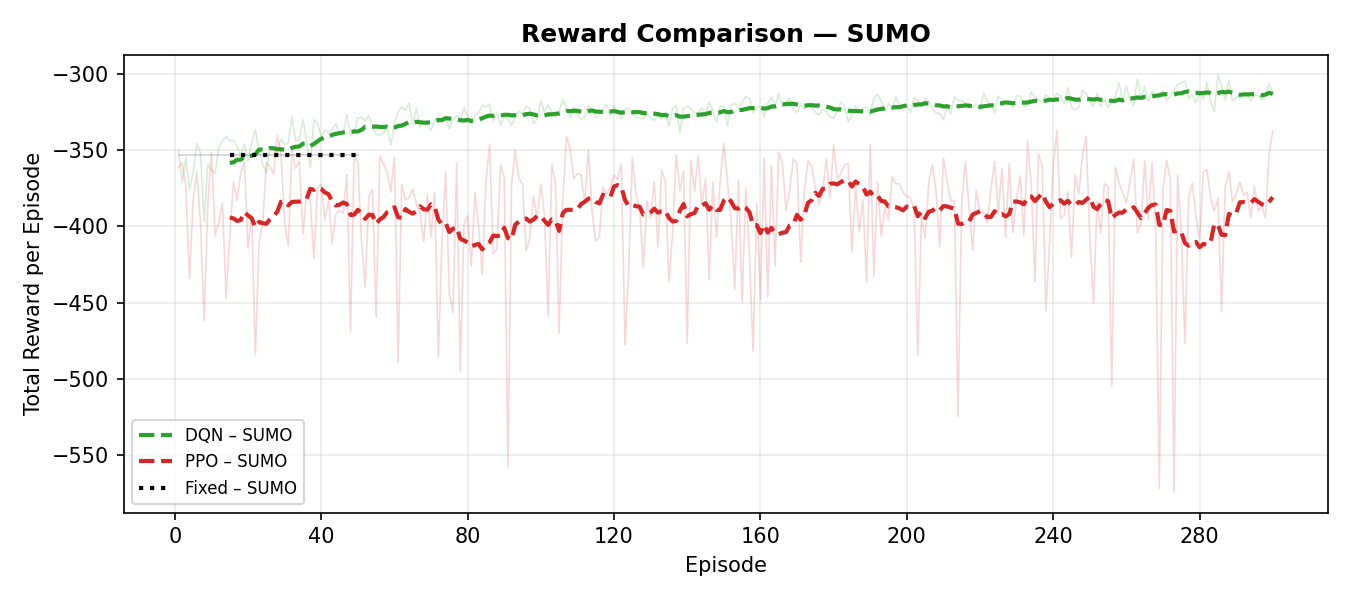
\includegraphics[width=0.60\textwidth]{results/comparison_sumo.png}
  \caption{Training reward curves on SUMO over 300 episodes.
  DQN converges steadily; PPO does not improve beyond the fixed baseline.}
  \label{fig:train_sumo}
\end{figure}

\begin{figure}[htbp]
  \centering
  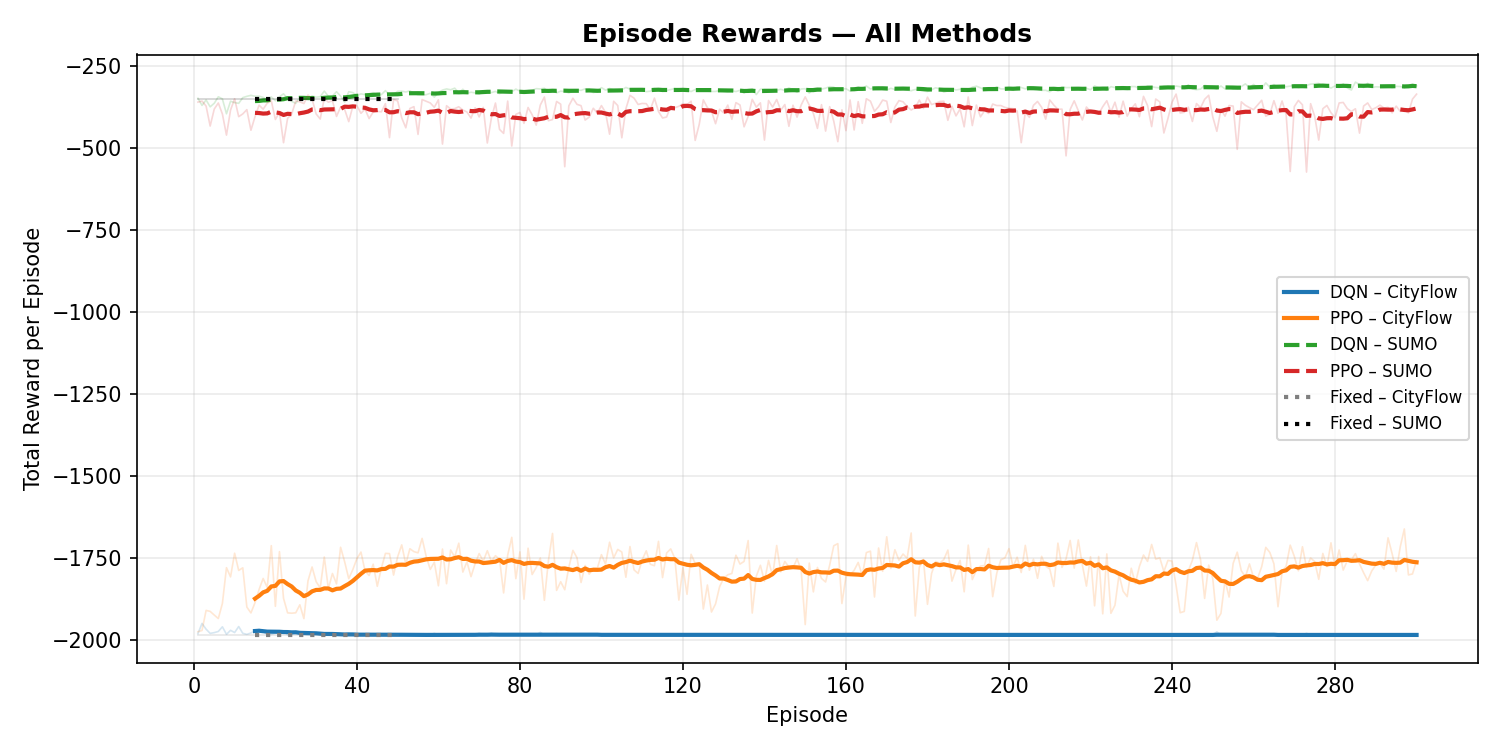
\includegraphics[width=0.60\textwidth]{results/comparison_rewards.png}
  \caption{Training reward curves on CityFlow over 300 episodes.
  PPO shows a gradual improvement; DQN remains near the fixed-time level.}
  \label{fig:train_cityflow}
\end{figure}

\subsection{Final Performance}

Table~\ref{tab:eval} reports evaluation metrics averaged over 10 held-out
episodes using the best saved checkpoint ($\varepsilon{=}0$ for DQN).

\begin{table}[htbp]
\centering
\caption{Evaluation results (10 episodes, best checkpoint).
Queue: mean waiting vehicles per step.
Throughput: vehicles completing their route per episode (SUMO only).}
\label{tab:eval}
\begin{tabular}{lrrrrr}
\toprule
 & \multicolumn{3}{c}{\textbf{SUMO}} & \multicolumn{2}{c}{\textbf{CityFlow}} \\
\cmidrule(lr){2-4}\cmidrule(lr){5-6}
\textbf{Method} & Reward & Queue & Throughput & Reward & Queue \\
\midrule
Fixed-time & $-352.9$ & $6.03$ & $1{,}018$ & $-1982.4$ & $449.6$ \\
DQN  & $\mathbf{-312.5}$ & $\mathbf{3.24}$ & $\mathbf{1{,}134}$ & $-1983.6$ & $446.6$ \\
PPO  & $-374.2$ & $7.60$ & $1{,}112$ & $\mathbf{-1791.9}$ & $469.6$ \\
\bottomrule
\end{tabular}
\end{table}

The bar charts in Figures~\ref{fig:eval_sumo} and~\ref{fig:eval_cityflow}
visualise these results across all three metrics.

\begin{figure}[htbp]
  \centering
  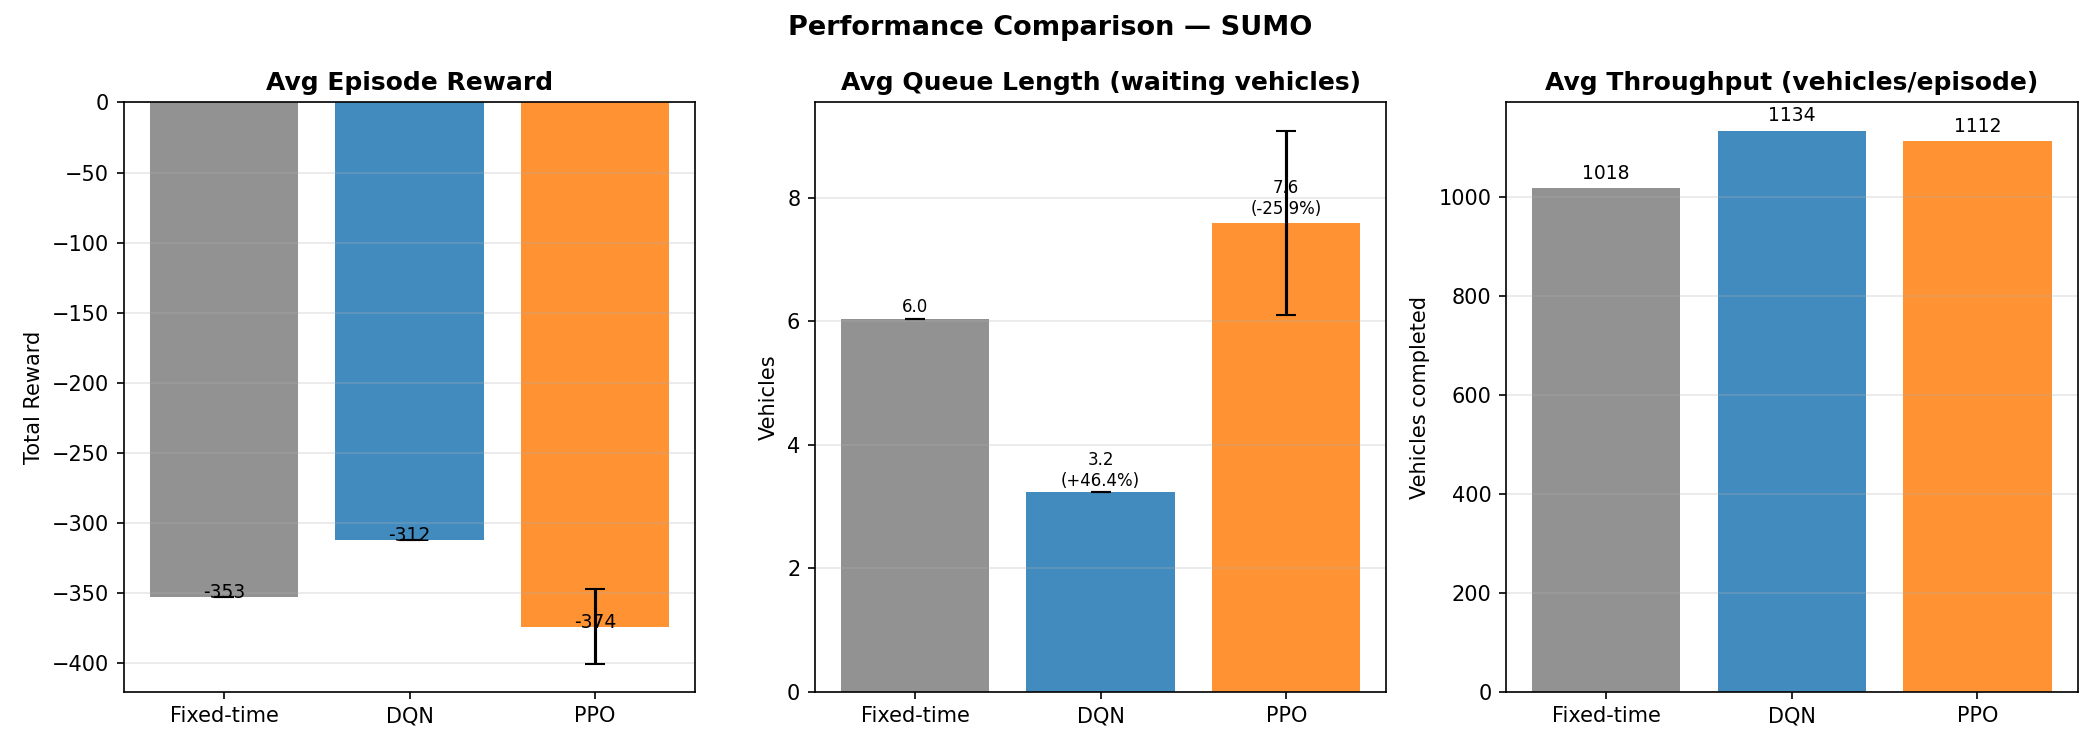
\includegraphics[width=0.65\textwidth]{results/evaluation_sumo.png}
  \caption{SUMO evaluation: average reward, queue length, and throughput
  per method.  DQN achieves the best score on all three metrics.}
  \label{fig:eval_sumo}
\end{figure}

\begin{figure}[htbp]
  \centering
  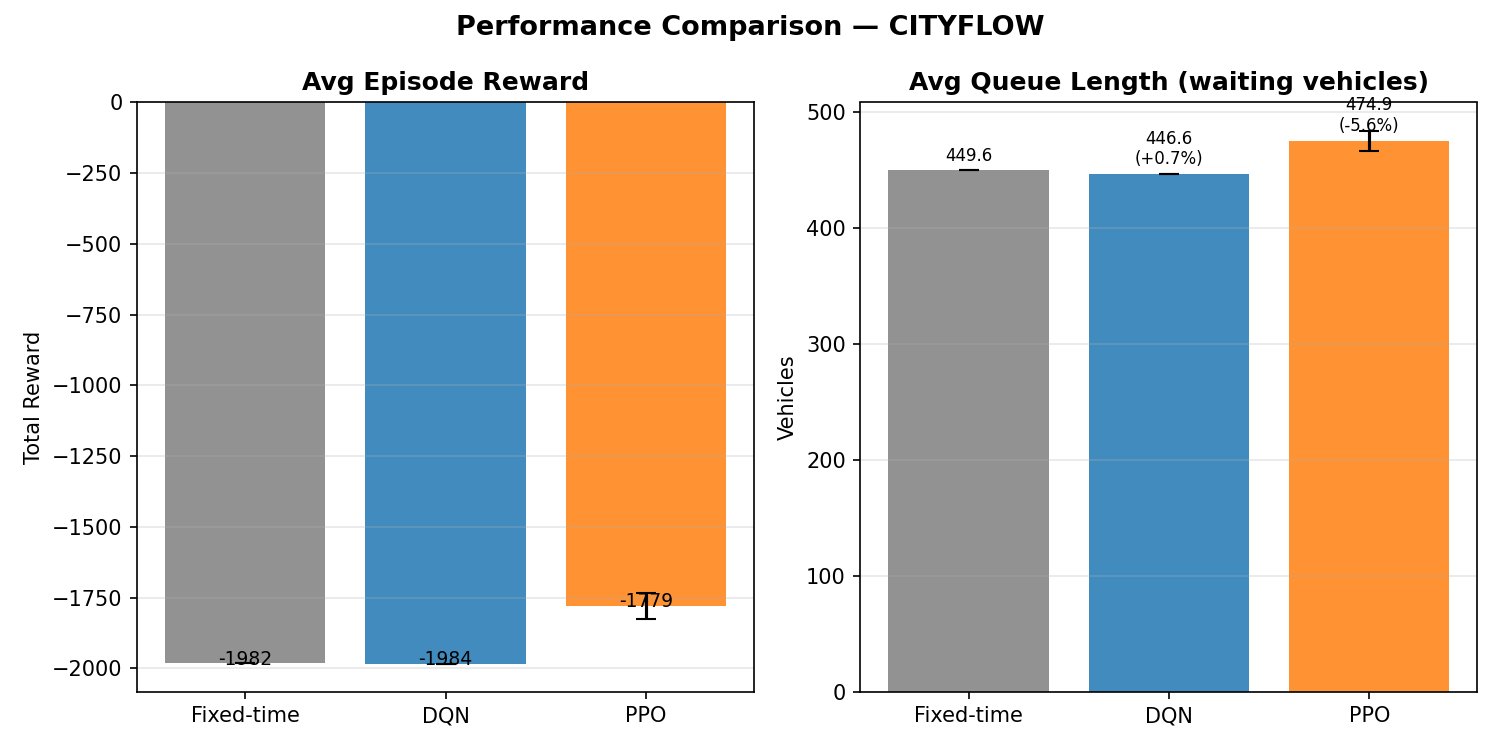
\includegraphics[width=0.65\textwidth]{results/evaluation_cityflow.png}
  \caption{CityFlow evaluation: average reward and queue length per method.
  PPO achieves the best reward; DQN is comparable to the fixed baseline.}
  \label{fig:eval_cityflow}
\end{figure}

\paragraph{SUMO.}
DQN achieves a \textbf{11.4\%} reward improvement ($-312.5$ vs.\ $-352.9$),
a \textbf{46.3\%} reduction in queue length ($3.24$ vs.\ $6.03$), and an
\textbf{11.4\%} increase in throughput ($1{,}134$ vs.\ $1{,}018$).  The
policy holds the heavier-demand phase for longer and switches once the queue
clears — consistent with the max-pressure heuristic~\citep{wei2019presslight}.

PPO on SUMO underperforms the fixed baseline on both reward and queue.
The on-policy gradient requires more samples to explore the binary action
space; combined with high-variance rewards during early phase-switching,
it does not converge within 300 episodes.

\paragraph{CityFlow.}
DQN matches the fixed baseline; PPO achieves a \textbf{9.6\%} reward gain.
The much higher absolute queues (${\sim}450$ vs.\ ${\sim}6$ on SUMO) indicate
near-saturation conditions where the binary action space cannot express
fine-grained splits, limiting the headroom for any adaptive policy.

\subsection{Signal Phase Analysis}

Figure~\ref{fig:phases} shows phase decisions over 200 steps for one
representative SUMO episode.  The fixed controller alternates rigidly every
30 steps.  DQN holds phases adaptively — longer when demand is heavy, shorter
when the queue clears.  PPO switches frequently within single action periods,
incurring yellow-transition overhead that reduces effective green time.

\begin{figure}[htbp]
  \centering
  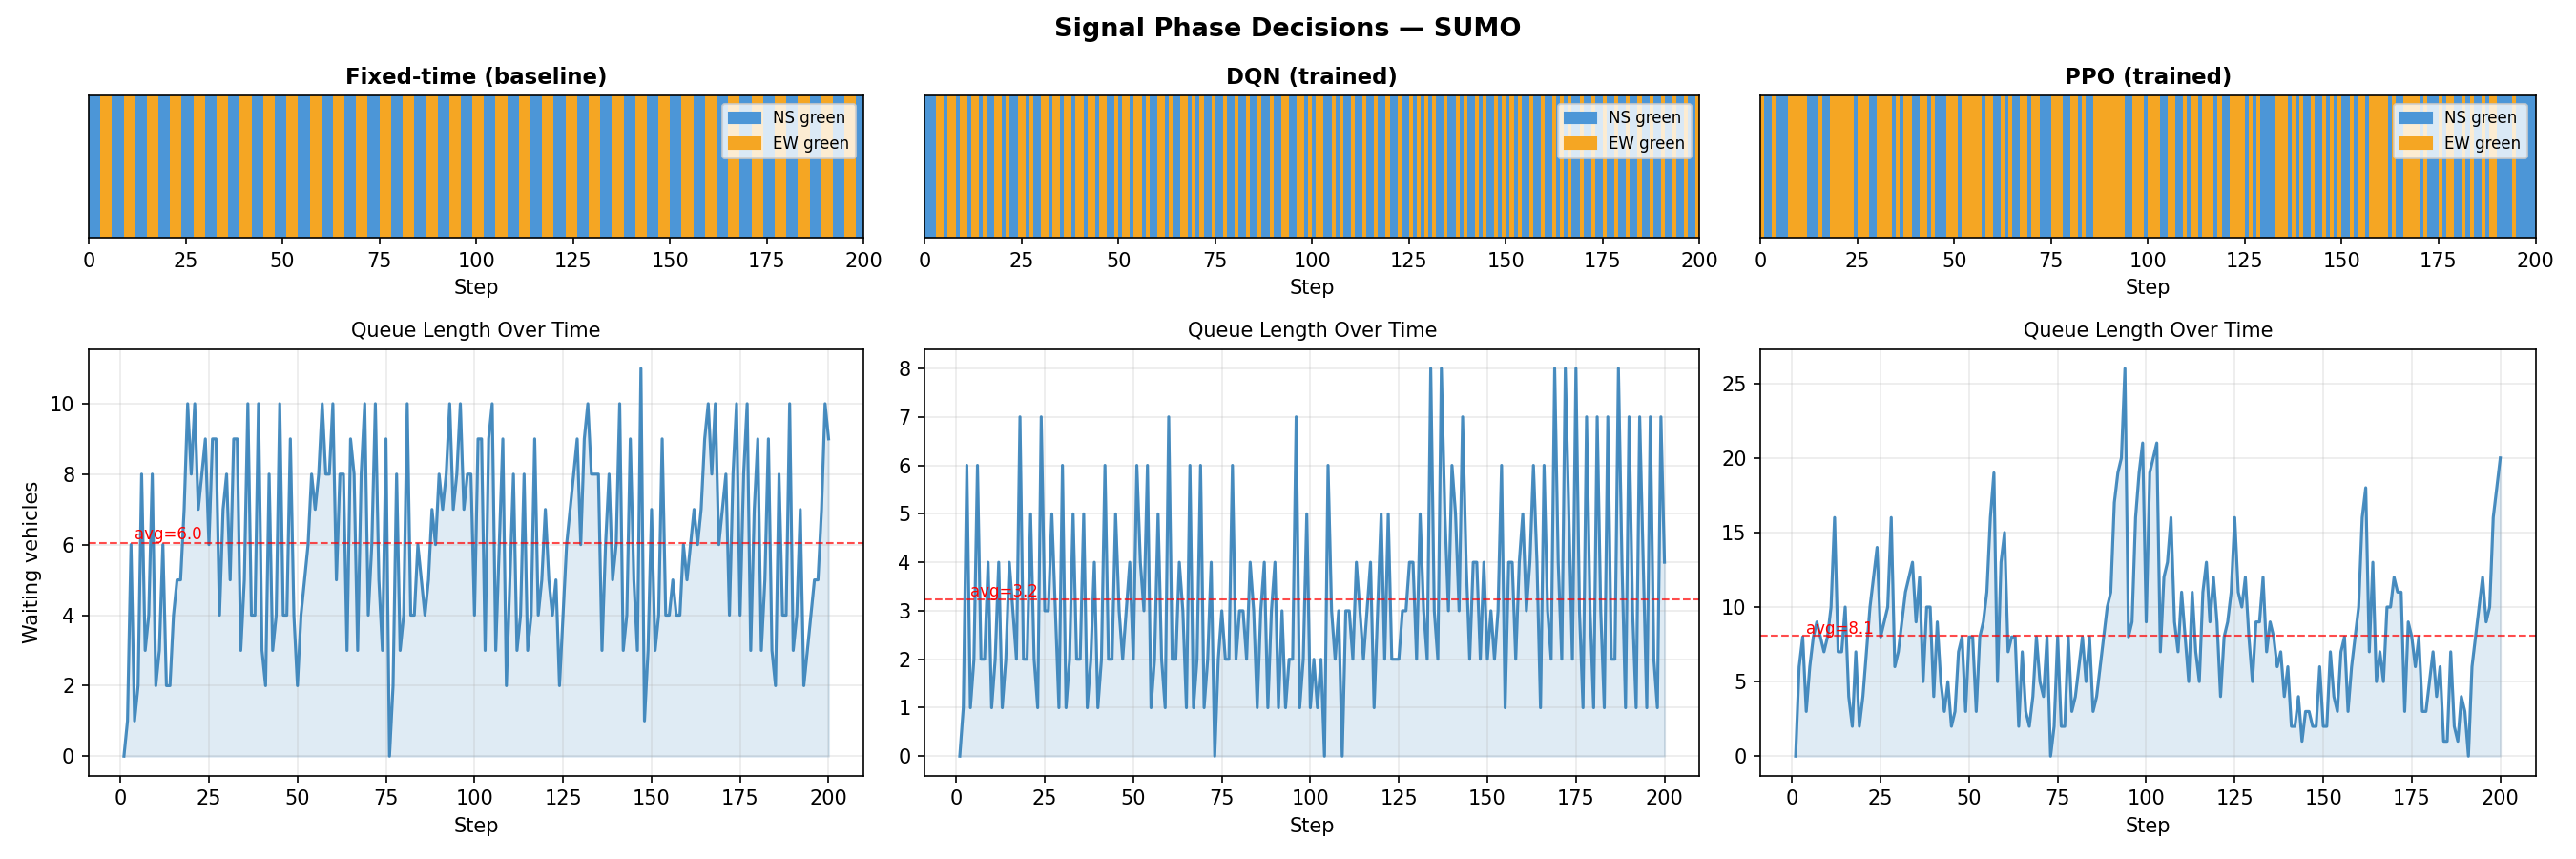
\includegraphics[width=0.72\textwidth]{results/phase_timeline_sumo.png}
  \caption{Signal phase decisions and queue traces over 200 steps (SUMO).
  \textbf{Top}: fixed-time (uniform 30-step periods).
  \textbf{Middle}: DQN (demand-adaptive, holds dominant direction longer).
  \textbf{Bottom}: PPO (high switching frequency).}
  \label{fig:phases}
\end{figure}

% ── 5. Conclusion ─────────────────────────────────────────────────────────────
\section{Conclusion}

On SUMO, Double Dueling DQN reduces queue length by 46\% and increases
throughput by 11\% over fixed-time control, demonstrating that deep RL
discovers non-trivial adaptive strategies from raw simulation experience.
On CityFlow's near-saturated scenario, PPO outperforms DQN, suggesting the
optimal algorithm depends on the traffic utilisation regime.

\paragraph{Limitations.}
Experiments cover a single isolated intersection with symmetric demand and a
binary action space that cannot express fractional green splits or more than
two phases.

\paragraph{Future work.}
\begin{itemize}
  \item \textbf{Multi-intersection MARL}: extend to a grid with graph
        attention coordination~\citep{wei2019colight}.
  \item \textbf{Variable phase durations}: allow the agent to also control
        how long each green phase lasts, not just which phase to serve.
  \item \textbf{Pressure reward}: replace Equation~\ref{eq:reward} to improve
        convergence under saturation conditions.
  \item \textbf{Real-world validation}: calibrate demand from loop-detector
        logs to test the approach on field data.
\end{itemize}

\acks{Code: \url{https://github.com/ashzyc/CS9170-RL-Traffic-Efficiency}.
All experiments were run on a standard laptop CPU; no external funding was received.}

\bibliography{references}

\end{document}
